\subsection{Configuração com 1 servidor WEB}

\paragraphnl{Resultados obtidos}

São apresentados em seguida sob a forma de uma tabela e de um gráfico os dados recolhidos para a configuração do serviço com um servidor web, nomeadamente o número de pedidos por segundos (débito) e a percentagem de pedidos falhados.

\begin{table}[!h]
\centering
\begin{tabular}{|c|c|c|}
\hline
\textbf{\# Clientes} & \textbf{Pedidos/s} & \textbf{\% Pedidos Falhados} \\ \hline
1 & 21.30 & 0 \\ \hline
2 & 25.42 & 0 \\ \hline
4 & 25.62 & 0 \\ \hline
8 & 26.41 & 0 \\ \hline
16 & 26.64 & 0 \\ \hline
32 & 24.03 & 0 \\ \hline
64 & 17.76 & 0 \\ \hline
128 & 12.28 & 23 \\ \hline
\end{tabular}
\caption{Tabela com débito e percentagem de pedidos falhados em função do número de clientes (1 Web Server)}
\end{table}

\begin{figure}[!h]
\centering
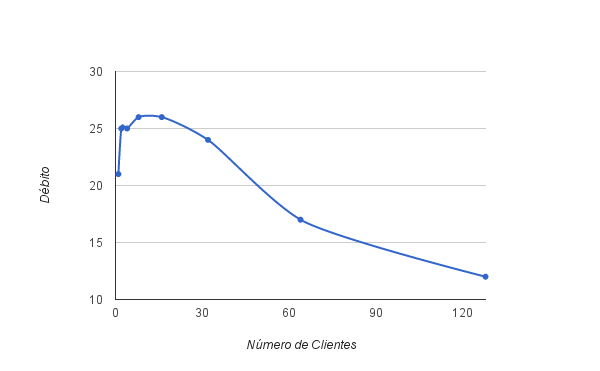
\includegraphics[scale=.6]{img/ab/web1.png}
\caption{Débito obtido de acordo com o número de clientes (1 Web Server)}
\end{figure}

\paragraphnl{Análise dos resultados anteriores}


\subsection{Configuração com 2 servidores WEB}

\paragraphnl{Resultados obtidos}

\begin{tabular}{|c|c|c|}
\hline
\textbf{\# Clientes} & \textbf{Pedidos/s} & \textbf{\% Pedidos Falhados} \\ \hline
1 & 24.45 & 0 \\ \hline
2 & 47.54 & 0 \\ \hline
4 & 51.02 & 0 \\ \hline
8 & 48.16 & 0 \\ \hline
16 & 49.47 & 0 \\ \hline
32 & 25.32 & 0 \\ \hline
64 & 19.20 & 0 \\ \hline
128 & 28.74 & 30 \\ \hline
256 & 39.17 & 34 \\ \hline
\end{tabular}

\paragraphnl{Análise dos resultados anteriores}
asdasd

\subsection{Configuração com 3 servidores WEB}

\paragraphnl{Resultados obtidos}

\begin{tabular}{|c|c|c|}
\hline
\textbf{\# Clientes} & \textbf{Pedidos/s} & \textbf{\% Pedidos Falhados} \\ \hline
1 & 25.18 & 0 \\ \hline
2 & 49.00 & 0 \\ \hline
4 & 43.94 & 0 \\ \hline
8 & 64.05 & 0 \\ \hline
16 & 62.30 & 0 \\ \hline
32 & 29.43 & 0 \\ \hline
64 & 43.57 & 0 \\ \hline
128 & 31.41 & 0 \\ \hline
256 & 28.51 & 0 \\ \hline
512 & 43.40 & 47 \\ \hline
\end{tabular}

\paragraphnl{Análise dos resultados anteriores}


\subsection{Configuração com 4 servidores WEB}

\paragraphnl{Resultados obtidos}

\begin{tabular}{|c|c|c|}
\hline
\textbf{\# Clientes} & \textbf{Pedidos/s} & \textbf{\% Pedidos Falhados} \\ \hline
1 & 25.79 & 0 \\ \hline
2 & 46.58 & 0 \\ \hline
4 & 68.22 & 0 \\ \hline
8 & 64.25 & 0 \\ \hline
16 & 66.57 & 0 \\ \hline
32 & 69.28 & 0 \\ \hline
64 & 46.27 & 0 \\ \hline
128 & 58.63 & 0 \\ \hline
256 & 34.06 & 0 \\ \hline
512 & 44.95 & 8 \\ \hline

\end{tabular}

\paragraphnl{Análise dos resultados anteriores}
olalalala


\subsection{Configuração com 6 servidores WEB}

\paragraphnl{Resultados obtidos}

\begin{tabular}{|c|c|c|}
\hline
\textbf{\# Clientes} & \textbf{Pedidos/s} & \textbf{\% Pedidos Falhados} \\ \hline
1 & 19.06 & 0 \\ \hline
2 & 34.40 & 0 \\ \hline
4 & 15.95 & 0 \\ \hline
8 & 50.40 & 0 \\ \hline
16 & 57.85 & 0 \\ \hline
32 & 57.04 & 0 \\ \hline
64 & 26.83 & 0 \\ \hline
128 & 18.01 & 0 \\ \hline
256 & 33.70 & 0 \\ \hline
512 & 45.13 & 7 \\ \hline

\end{tabular}

\paragraphnl{Análise dos resultados anteriores}
olalalala
